% Options for packages loaded elsewhere
\PassOptionsToPackage{unicode}{hyperref}
\PassOptionsToPackage{hyphens}{url}
%
\documentclass[
  10pt,
]{scrbook}
\usepackage{amsmath,amssymb}
\usepackage{lmodern}
\usepackage{iftex}
\ifPDFTeX
  \usepackage[T1]{fontenc}
  \usepackage[utf8]{inputenc}
  \usepackage{textcomp} % provide euro and other symbols
\else % if luatex or xetex
  \usepackage{unicode-math}
  \defaultfontfeatures{Scale=MatchLowercase}
  \defaultfontfeatures[\rmfamily]{Ligatures=TeX,Scale=1}
  \setmainfont[]{Source Serif Pro}
  \setsansfont[]{Source Sans Pro}
  \setmonofont[Scale=0.8]{Source Code Pro}
\fi
% Use upquote if available, for straight quotes in verbatim environments
\IfFileExists{upquote.sty}{\usepackage{upquote}}{}
\IfFileExists{microtype.sty}{% use microtype if available
  \usepackage[]{microtype}
  \UseMicrotypeSet[protrusion]{basicmath} % disable protrusion for tt fonts
}{}
\makeatletter
\@ifundefined{KOMAClassName}{% if non-KOMA class
  \IfFileExists{parskip.sty}{%
    \usepackage{parskip}
  }{% else
    \setlength{\parindent}{0pt}
    \setlength{\parskip}{6pt plus 2pt minus 1pt}}
}{% if KOMA class
  \KOMAoptions{parskip=half}}
\makeatother
\usepackage{xcolor}
\IfFileExists{xurl.sty}{\usepackage{xurl}}{} % add URL line breaks if available
\IfFileExists{bookmark.sty}{\usepackage{bookmark}}{\usepackage{hyperref}}
\hypersetup{
  pdftitle={LaTeX Dersleri},
  pdfauthor={Zafer Acar},
  hidelinks,
  pdfcreator={LaTeX via pandoc}}
\urlstyle{same} % disable monospaced font for URLs
\usepackage{color}
\usepackage{fancyvrb}
\newcommand{\VerbBar}{|}
\newcommand{\VERB}{\Verb[commandchars=\\\{\}]}
\DefineVerbatimEnvironment{Highlighting}{Verbatim}{commandchars=\\\{\}}
% Add ',fontsize=\small' for more characters per line
\usepackage{framed}
\definecolor{shadecolor}{RGB}{248,248,248}
\newenvironment{Shaded}{\begin{snugshade}}{\end{snugshade}}
\newcommand{\AlertTok}[1]{\textcolor[rgb]{0.94,0.16,0.16}{#1}}
\newcommand{\AnnotationTok}[1]{\textcolor[rgb]{0.56,0.35,0.01}{\textbf{\textit{#1}}}}
\newcommand{\AttributeTok}[1]{\textcolor[rgb]{0.77,0.63,0.00}{#1}}
\newcommand{\BaseNTok}[1]{\textcolor[rgb]{0.00,0.00,0.81}{#1}}
\newcommand{\BuiltInTok}[1]{#1}
\newcommand{\CharTok}[1]{\textcolor[rgb]{0.31,0.60,0.02}{#1}}
\newcommand{\CommentTok}[1]{\textcolor[rgb]{0.56,0.35,0.01}{\textit{#1}}}
\newcommand{\CommentVarTok}[1]{\textcolor[rgb]{0.56,0.35,0.01}{\textbf{\textit{#1}}}}
\newcommand{\ConstantTok}[1]{\textcolor[rgb]{0.00,0.00,0.00}{#1}}
\newcommand{\ControlFlowTok}[1]{\textcolor[rgb]{0.13,0.29,0.53}{\textbf{#1}}}
\newcommand{\DataTypeTok}[1]{\textcolor[rgb]{0.13,0.29,0.53}{#1}}
\newcommand{\DecValTok}[1]{\textcolor[rgb]{0.00,0.00,0.81}{#1}}
\newcommand{\DocumentationTok}[1]{\textcolor[rgb]{0.56,0.35,0.01}{\textbf{\textit{#1}}}}
\newcommand{\ErrorTok}[1]{\textcolor[rgb]{0.64,0.00,0.00}{\textbf{#1}}}
\newcommand{\ExtensionTok}[1]{#1}
\newcommand{\FloatTok}[1]{\textcolor[rgb]{0.00,0.00,0.81}{#1}}
\newcommand{\FunctionTok}[1]{\textcolor[rgb]{0.00,0.00,0.00}{#1}}
\newcommand{\ImportTok}[1]{#1}
\newcommand{\InformationTok}[1]{\textcolor[rgb]{0.56,0.35,0.01}{\textbf{\textit{#1}}}}
\newcommand{\KeywordTok}[1]{\textcolor[rgb]{0.13,0.29,0.53}{\textbf{#1}}}
\newcommand{\NormalTok}[1]{#1}
\newcommand{\OperatorTok}[1]{\textcolor[rgb]{0.81,0.36,0.00}{\textbf{#1}}}
\newcommand{\OtherTok}[1]{\textcolor[rgb]{0.56,0.35,0.01}{#1}}
\newcommand{\PreprocessorTok}[1]{\textcolor[rgb]{0.56,0.35,0.01}{\textit{#1}}}
\newcommand{\RegionMarkerTok}[1]{#1}
\newcommand{\SpecialCharTok}[1]{\textcolor[rgb]{0.00,0.00,0.00}{#1}}
\newcommand{\SpecialStringTok}[1]{\textcolor[rgb]{0.31,0.60,0.02}{#1}}
\newcommand{\StringTok}[1]{\textcolor[rgb]{0.31,0.60,0.02}{#1}}
\newcommand{\VariableTok}[1]{\textcolor[rgb]{0.00,0.00,0.00}{#1}}
\newcommand{\VerbatimStringTok}[1]{\textcolor[rgb]{0.31,0.60,0.02}{#1}}
\newcommand{\WarningTok}[1]{\textcolor[rgb]{0.56,0.35,0.01}{\textbf{\textit{#1}}}}
\usepackage{longtable,booktabs,array}
\usepackage{calc} % for calculating minipage widths
% Correct order of tables after \paragraph or \subparagraph
\usepackage{etoolbox}
\makeatletter
\patchcmd\longtable{\par}{\if@noskipsec\mbox{}\fi\par}{}{}
\makeatother
% Allow footnotes in longtable head/foot
\IfFileExists{footnotehyper.sty}{\usepackage{footnotehyper}}{\usepackage{footnote}}
\makesavenoteenv{longtable}
\usepackage{graphicx}
\makeatletter
\def\maxwidth{\ifdim\Gin@nat@width>\linewidth\linewidth\else\Gin@nat@width\fi}
\def\maxheight{\ifdim\Gin@nat@height>\textheight\textheight\else\Gin@nat@height\fi}
\makeatother
% Scale images if necessary, so that they will not overflow the page
% margins by default, and it is still possible to overwrite the defaults
% using explicit options in \includegraphics[width, height, ...]{}
\setkeys{Gin}{width=\maxwidth,height=\maxheight,keepaspectratio}
% Set default figure placement to htbp
\makeatletter
\def\fps@figure{htbp}
\makeatother
\setlength{\emergencystretch}{3em} % prevent overfull lines
\providecommand{\tightlist}{%
  \setlength{\itemsep}{0pt}\setlength{\parskip}{0pt}}
\setcounter{secnumdepth}{5}
\usepackage[turkish,shorthands=:!]{babel}
\usepackage{amsmath,amsfonts,amssymb,amsthm}
\usepackage{tabularx}
\makeatletter
\def\thm@space@setup{%
  \thm@preskip=8pt plus 2pt minus 4pt
  \thm@postskip=\thm@preskip
}
\makeatother

\renewcommand{\textfraction}{0.05}
\renewcommand{\topfraction}{0.8}
\renewcommand{\bottomfraction}{0.8}
\renewcommand{\floatpagefraction}{0.75}

\usepackage{booktabs}
\usepackage{longtable}
\usepackage[bf]{caption}

\usepackage{framed,color}

\renewcommand{\href}[2]{#2\footnote{\url{#1}}}


\usepackage{makeidx}
\makeindex


\frontmatter
\ifLuaTeX
  \usepackage{selnolig}  % disable illegal ligatures
\fi
\usepackage[]{natbib}
\bibliographystyle{apalike}

\title{LaTeX Dersleri}
\author{Zafer Acar}
\date{2022-01-21}

\begin{document}
\maketitle



{
\setcounter{tocdepth}{2}
\tableofcontents
}
\listoffigures
\listoftables
\hypertarget{uxf6nsuxf6z}{%
\chapter*{Önsöz}\label{uxf6nsuxf6z}}


\mainmatter

\hypertarget{genel}{%
\chapter{Genel}\label{genel}}

Bu bölümde LaTeX kullanımıyla ilgili genel bilgilerden bahsedeceğiz.

\hypertarget{latex-nedir}{%
\section{LaTeX Nedir?}\label{latex-nedir}}

Önce TeX'le başlayalım. TeX, 1978'den
itibaren \href{https://www-cs-faculty.stanford.edu/~knuth/}{Donald Knuth} tarafından belgelerin bilgisayarda dizilmesi
için geliştirdiği bir dizgi sistemidir.
LaTeX ise TeX'in kullanımını kolaylaştırmak için 1984 yılında \href{http://www.lamport.org/}{Leslie
Lamport} tarafından tasarlanmış bir makro pakettir.

LaTeX, genelde WYSIWYG\footnote{WYSIWYG, İngilizce'de ``What You See Is What You Get'' teriminin baş harflerinden oluşan bir bilgisayar terimidir. Türkçesi \emph{Ne Görüyorsan Onu Alırsın} demek olup ekranda görülene çok benzer bir çıktı alınacağı ortamları tanımlar.} editörleriyle karşılaştırılır. WYSIWYG, Microsoft
Word, Libreoffice Writer gibi kelime işlemcilere ya da Adobe Indesign
gibi programlara verilen genel bir isimdir. Hepsinin ortak özelliği,
girdi ile çıktının aynı anda ve birlikte görünmesidir.

Bir metnin genel görünümü ve okunabilirliği, metnin nasıl
hizalandığından ve kesildiğinden büyük ölçüde etkilenir. LaTeX, tüm
paragraf için hizalamayı ve kesmeleri optimize eden son derece gelişmiş
TeX algoritmalarını kullanır. Kelime işlemciler ve diğer programlar,
satır başına çalıştıkları için oldukça yetersiz kalırlar. Bu, diğer
şeylerin yanı sıra düzensiz aralıklara ve birçok kısa çizgiye sebep
olur. Sonuçları görmeniz için Microsoft Word 2008 (Mac), Adobe InDesign
CS4 ve LaTeX'le dizilmiş bir metni \href{http://www.rtznet.nl/zink/comparison.pdf}{şuradan} inceleyebilirsiniz.

Sonuç, LaTeX'in diğer programların her ikisinden de üstün olduğunu
açıkça gösterir: iki kat daha az tireleme kullanır ve yine de sözcük
aralığındaki varyasyon, Word veya InDesign'dan belirgin şekilde daha
azdır. LaTeX'te çok büyük sözcük aralığı içeren satırlar oluşmaz.

LaTeX'de girdi ve çıktı ekranı farklıdır ve
çıktıyı görmek için girdinin derleme işleminden geçmesi gerekir. Ayrıca
birçok şey için WYSIWYG editörlerinde olmayan yapılar vardır. Şimdi, bu
yapıların ne oldukları ve ne işe yaradıklarını açıklayalım.

\hypertarget{uxf6nemli-yapux131lar}{%
\section{Önemli Yapılar}\label{uxf6nemli-yapux131lar}}

\hypertarget{komutlar}{%
\subsection{Komutlar}\label{komutlar}}

LaTeX komutları bir geribölü (\texttt{\textbackslash{}}) işaretiyle başlar ve ya sadece
harflerden ya da bir tane harf olmayan karakterden oluşurlar. Komut
yazıldıktan sonra ya boşluk, ya bir sayı ya da harf olmayan bir karakter
gelebilir.

Çoğu komut, zorunlu değişken alır. Bu zorunlu değişken komut adından
sonra çengelli parantezler içine yazılır. Zorunlu değişken alan
komutlar, zorunlu olmayan (isteğe bağlı) değişkenler de alabilir, bunlar
da komut adından sonra gelen köşeli parantezler içine yazılırlar. Eğer
değişkenler birden fazlaysa aralarına virgül koyularak ayrılır.

\begin{Shaded}
\begin{Highlighting}[numbers=left,,]
\NormalTok{\textbackslash{}}\SpecialCharTok{:}
\NormalTok{\textbackslash{}LaTeX}
\NormalTok{\textbackslash{}item[...]}
\NormalTok{\textbackslash{}emph\{...\}}
\NormalTok{\textbackslash{}documentclass[...]\{...\}}
\NormalTok{\textbackslash{}subfloat[...][...]\{...\}}
\NormalTok{\textbackslash{}raisebox\{...\}[...][...]\{...\}}
\NormalTok{\textbackslash{}multicolumn\{...\}\{...\}\{...\}}
\NormalTok{\{\textbackslash{}bfseries ...\}}
\end{Highlighting}
\end{Shaded}

Fikir vermesi açısından yukarıda dokuz adet komut örneği verilmiştir.
Birinci komut bir tane harf olmayan karakterden oluşan bir komuttur.
İkincisi, değişkeni olmayan bir komuttur. Bazı harflerin büyük
bazılarınınsa küçük olması komutların büyük-küçük harfe duyarlı olduğunu
gösterir. Dokuzuncu komut ise bildirim şeklinde verilmiştir.

\hypertarget{paketler}{%
\subsection{Paketler}\label{paketler}}

LaTeX'de bazı özelliklerin (renkli yazmak, şekil eklemek vb.)
kullanılabilmesi için kaynak dosyaya bazı paketlerin eklenmesi gerekir.
Bu, \texttt{\textbackslash{}usepackage} komutuyla yapılır. Bu komutun zorunlu değişkenine
paket adı, zorunlu olmayan kısmına ise paket seçenekleri yazılır:

\begin{Shaded}
\begin{Highlighting}[]
\NormalTok{\textbackslash{}usepackage[}\SpecialCharTok{\textless{}}\NormalTok{seçenekler}\SpecialCharTok{\textgreater{}}\NormalTok{]\{}\SpecialCharTok{\textless{}}\NormalTok{paket adı}\SpecialCharTok{\textgreater{}}\NormalTok{\}}
\end{Highlighting}
\end{Shaded}

Bu komutla paketin kaynak dosyaya eklenmesi TeX dağıtımıyla sisteminize
kurulmuş olan paketin belgeye çağrılarak işe koşulması demektir.

\hypertarget{ortamlar}{%
\subsection{Ortamlar}\label{ortamlar}}

LaTeX'de ortamlar önemli bir yer tutar. Örneğin \texttt{document} bir ortamdır.
Ortamları birden fazla ögeye uygulanan komutlar olarak düşünebiliriz.

Bir ortam \texttt{\textbackslash{}begin} komutuyla başlayıp \texttt{\textbackslash{}end} komutuyla biter. Her iki
komutun zorunlu değişkeni ortamın adıdır:

\begin{Shaded}
\begin{Highlighting}[]
\NormalTok{\textbackslash{}begin\{}\SpecialCharTok{\textless{}}\NormalTok{ortam adı}\SpecialCharTok{\textgreater{}}\NormalTok{\}}
\NormalTok{ ...}
\NormalTok{\textbackslash{}end\{}\SpecialCharTok{\textless{}}\NormalTok{ortam adı}\SpecialCharTok{\textgreater{}}\NormalTok{\}}
\end{Highlighting}
\end{Shaded}

\hypertarget{gruplar}{%
\subsection{Gruplar}\label{gruplar}}

Gruplar, ortam benzeri yapılardır. Grup \texttt{\textbackslash{}begingroup} komutuyla başlar
ve \texttt{\textbackslash{}endgroup} komutuyla biter. Grubun içinde kullanılan bir bildirim
sadece gruba uygulanır.

\hypertarget{bosluk}{%
\subsection{Boşluklar}\label{bosluk}}

LaTeX'de belgenizin metnini oluştururken ister klavyedeki Space, ister
Tab tuşu ile boşluk bırakın, bu boşluklar LaTeX tarafından bir karakter
boşluk olarak algılanır. Arka arkaya çok sayıda boşluk bırakılsa da
LaTeX bunu tek bir boşluk olarak algılar.

Bütün bir satırın boş bırakılması LaTeX tarafından paragraf başı olarak
algılanır. Arka arkaya boş bırakılan çok sayıda boş satır LaTeX
tarafından tek bir boş satır yani paragraf başı olarak algılanır.

\begin{Shaded}
\begin{Highlighting}[]
\NormalTok{ İster bir boşluk, isterseniz de çok         sayıda boşluk bırakın. }
\NormalTok{İkisi de bir boşluk gibi işlem görür. }

\NormalTok{Boş bir satır yeni paragraf demektir, burada olduğu gibi.}
\end{Highlighting}
\end{Shaded}

\href{https://github.com/acarzfr/latex-dersleri/blob/main/examples/ex1.pdf}{Çıktı}

Komutlardan sonra gelen boşlukları LaTeX dikkate almaz. Komuttan sonra
gerçekten bir boşluk bırakmak için, ya \texttt{\{\}} ve ardından boşluk girilir
ya da komut adından sonra özel bir boşluk komutu kullanılır.

\begin{Shaded}
\begin{Highlighting}[]
\NormalTok{\textbackslash{}LaTeX  boşluk yok.\textbackslash{}\textbackslash{}}
\NormalTok{\textbackslash{}LaTeX\{\} boşluk var.\textbackslash{}\textbackslash{}}
\NormalTok{\textbackslash{}LaTeX\textbackslash{} boşluk komutuyla  boşluk.}
\end{Highlighting}
\end{Shaded}

\href{https://github.com/acarzfr/latex-dersleri/blob/main/examples/ex2.pdf}{Çıktı}

\hypertarget{uxf6zel-amauxe7lux131-karakterler}{%
\subsection{Özel amaçlı karakterler}\label{uxf6zel-amauxe7lux131-karakterler}}

Aşağıdaki karakterlerin herbiri LaTeX'de özel bir amaç için kullanılır.
Dolayısıyla bu karakterleri doğrudan kullanmak istenmeyen sonuçlara yol
açabilir.

\begin{Shaded}
\begin{Highlighting}[]
\CommentTok{\#  $  \%   \&   \{   \}   \textasciitilde{}  \^{}  \_ \textbackslash{}}
\end{Highlighting}
\end{Shaded}

Bu karakterleri çıktıda elde etmek isterseniz, sondaki hariç, başına bir
geribölü koymanız gerekir. Sondaki için, yani bir geribölü sembolü elde
etmek içinse \texttt{\textbackslash{}textbackslash} komutunu kullanabilirsiniz. Eğer \texttt{\textbackslash{}\textbackslash{}}
komutunu verirseniz yeni bir satır başlatmış olursunuz.

Bu karakterlerden örneğin yüzde (\texttt{\%}) karakteri kaynak dosyanızda yorum
ya da açıklama yazmaya yarar. Bu sembolden sonra yazılanları LaTeX
dikkate almaz ve çıktıda görünmez.

Diğer karakterlerden örneğin (\texttt{\$}) nin matematik kipini açma ve
kapatmaya yarar. (\texttt{\&}) karekteri tablo ve benzeri yapılarda dikey
hizalama yapmak için veya sütun ayracı olarak kullanılır. Çengelli
parantezlerden zaten yeterince bahsettik. (\texttt{\#}) karakteri yeni komutlar
tanımlamakta kullanılır. Tilda (\texttt{\textasciitilde{}}) ise genişlemeyen bir boşluk
yaratmak için kullanılır. (\texttt{\^{}}) ve (\texttt{\_}) karakterleri de matematikte üst
ve alt indis yazmak için kullanılır. Her birinin kullanımlarından yeri
geldiğinde tekrar bahsedeceğiz.

\hypertarget{kurulum}{%
\section{Kurulum}\label{kurulum}}

LaTeX'i kurmak için ilk olarak bir TeX dağıtımı edinmeniz gerekir.
Dağıtımlar, dizgi sistemini ve LaTeX'de belge oluşturabilmek için
gereken paketleri içerir.

İkinci ihtiyaç duyacağınız şey bir LaTeX editörüdür. Edindiğiniz TeX
dağıtımları genelde bir LaTeX editörüyle birlikte gelir. Tabi editör
kişisel bir tercihtir ve bir LaTeX editörü yerine basit bir metin
editörü kullanabilirsiniz. Ancak farklı işletim sistemleri için birçok
iyi LaTeX editörü vardır ve bunların kod vurgulama, otomatik tamamlama,
otomatik belge oluşturma gibi LaTeX'e özgü işlevleri vardır. Dolayısıyla
LaTeX'de yeniyseniz bir editör kullanmanızı tavsiye ederiz.

\hypertarget{gnulinux}{%
\subsection{GNU/Linux}\label{gnulinux}}

Linux sistemlere \href{https://miktex.org/download}{MiKTeX} ya da \href{http://www.tug.org/texlive/}{TeX
Live} kurulabilir. MiKTeX'in indirme sayfasında Ubuntu, Mint,
Debian, Fedora, CentOS ve openSUSE gibi Linux dağıtımlarında nasıl
kurulacağı anlatılmıştır. TeX Live ise tüm popüler Linux dağıtımlarının
depolarında mevcut olup, paket yöneticisi ya da komut satırı yardımıyla
kurulabilir. Örneğin Ubuntu, Debian, Mint, Pardus gibi \texttt{.deb} uzantılı
paketlerin kullanıldığı dağıtımlarda

\begin{Shaded}
\begin{Highlighting}[]
\NormalTok{sudo apt}\SpecialCharTok{{-}}\NormalTok{get install texlive}\SpecialCharTok{{-}}\NormalTok{base}
\end{Highlighting}
\end{Shaded}

komutuyla temel kurulum,

\begin{Shaded}
\begin{Highlighting}[]
\NormalTok{sudo apt}\SpecialCharTok{{-}}\NormalTok{get install texlive}\SpecialCharTok{{-}}\NormalTok{full}
\end{Highlighting}
\end{Shaded}

komutuyla da tam kurulum yapılır.

\hypertarget{mac-os}{%
\subsection{Mac OS}\label{mac-os}}

Mac OS kullanıcıları için iki seçenek mevcuttur:
\href{https://miktex.org/download}{MiKTeX} ya da
\href{http://www.tug.org/mactex/}{MacTeX}. MiKTeX kurulumu için \texttt{.dmg} uzantılı, MacTeX içinse
\texttt{.pkg} uzantılı dosya indirilir ve standart kurulum yapılır.

\hypertarget{windows}{%
\subsection{Windows}\label{windows}}

Windows için aşağıdaki dağıtımlardan birini kurabilirsiniz.

\begin{itemize}
\tightlist
\item
  \href{https://miktex.org/download}{MiKTeX}
\item
  \href{http://www.tug.org/texlive/}{TeX Live}
\item
  \href{https://tug.org/protext/}{proTeXt}
\end{itemize}

MiKTeX veya TeX Live dağıtımını kurarsanız sisteminize
\href{https://www.tug.org/texworks/}{TeXworks} editörü de kurulur. proTeXt dağıtımı MiKTeX tabanlı bir
dağıtım olup, tüm paketleri içerir ve beraberinde
\href{https://texstudio.org/}{TeXstudio} editörüyle gelir.

\hypertarget{latex-edituxf6rleri}{%
\subsection{LaTeX Editörleri}\label{latex-edituxf6rleri}}

Hangi editörü kullanacağınıza birkaç deneme yaptıktan sonra karar
verebilirsiniz. \href{https://beebom.com/best-latex-editors/}{Burada} en çok
beğenilen editörler listelenmiş.

Her LaTeX editöründe olan özelliklerin (otomatik kod tamamlama vb.) yanı
sıra kullanıcı dostu arayüzü, yüzde yüze yakın Türkçe desteği, ücretsiz
oluşu ve her üç sistemde de çalışabilmesinden dolayı
\href{https://texstudio.org/}{TeXstudio}'yu tavsiye ediyoruz. Karar sizin.

\hypertarget{uxe7evrimiuxe7i-edituxf6rler}{%
\subsection{Çevrimiçi Editörler}\label{uxe7evrimiuxe7i-edituxf6rler}}

LaTeX'i hiçbir kurulum yapmadan çevrimiçi de kullanabilirsiniz. Aşağıda
üç tanesi listelenmiştir.

\begin{itemize}
\tightlist
\item
  \href{https://www.overleaf.com/}{Overleaf}
\item
  \href{https://papeeria.com/}{Papeeria}
\item
  \href{https://latexbase.com/}{LaTeX Base}
\end{itemize}

En popüler olanı Overleaf olup, sayfasında beğenebileceğiniz binlerce
\href{https://www.overleaf.com/latex/templates}{şablon} ve LaTeX kullanımına yönelik
\href{https://www.overleaf.com/learn}{anlatımlar} bulunur.

\hypertarget{tipik}{%
\section{Tipik Bir Belge Yazımı}\label{tipik}}

LaTeX'in varsayılan dosya uzantısı \texttt{.tex}'tir. Bu basit bir metin
dosyası olup, LaTeX editörleriyle oluşturulup düzenlenebileceği gibi
basit bir metin editörüyle de düzenlenebilir.

Bir belge hazırlamaya başlamak için verilecek ilk komut

\begin{Shaded}
\begin{Highlighting}[]
\NormalTok{\textbackslash{}documentclass[...]\{...\}}
\end{Highlighting}
\end{Shaded}

olup, çengelli parantezler arasına oluşturmak istediğiniz belgenin
sınıfı yazılır. Köşeli parantezlerin içine de isteğe bağlı bazı
değişkenler yazılabilir. Eğer bu kısım boş bırakılırsa LaTeX varsayılan
değerleri alacaktır. Bu komutun ardından sırasıyla \texttt{\textbackslash{}begin\{document\}} ve
\texttt{\textbackslash{}end\{document\}} komutları verilerek belge ortamı oluşturulur.
\texttt{\textbackslash{}end\{document\}} komutuyla LaTeX'e belgenin bittiği söylenmiş olur ve
LaTeX bu komuttan sonra girilenleri dikkate almaz.

\texttt{\textbackslash{}documentclass} komutuyla \texttt{\textbackslash{}begin\{document\}} komutu arasına \emph{sahanlık}
denir. Sahanlık, belgenin ayarlarının yapıldığı kısımdır ve bu kısım
çıktıda görünmez. \texttt{\textbackslash{}begin\{document\}} ile \texttt{\textbackslash{}end\{document\}} arasına da
\emph{gövde} denir. İçerik burada oluşturulur.

Aşağıda asgari bir LaTeX kaynak dosyası gösterilmiştir. \texttt{\textbackslash{}documentclass}
komutunun değişkeni olan \texttt{article}, belgenin makale olacağını belirtir.

\begin{Shaded}
\begin{Highlighting}[]
\NormalTok{\textbackslash{}documentclass\{article\}}
\NormalTok{\textbackslash{}begin\{document\}}
\NormalTok{İşte ilk belgem.}
\NormalTok{\textbackslash{}end\{document\}}
\end{Highlighting}
\end{Shaded}

Bu noktadan sonra örnek kaynak dosyayı LaTeX editörünüzünde oluşturup
önceden oluşturduğunuz bir dizine kaydedin. Kaydederken dosya adında
boşluk ve Türkçe karakter kullanmayın. Örneğin kaynak dosyanız
\texttt{belge1.tex} olsun.

İkinci aşama kaynak dosyanın derlenmesidir. Derleme işlemi için LaTeX
editörlerinde genelde araç çubuğunda oklar bulunur. Oka tıklandığında
dosya derlenir ve sonuç, çıktı ekranında görünür.

Eğer metin editörü kullanıyorsanız derlemeyi uçbirimde (terminal,
konsol,\ldots) yapmanız gerekir. Derleme için uçbirim kaynak dosyanın
olduğu dizinde açılıp

\begin{Shaded}
\begin{Highlighting}[]
\NormalTok{pdflatex belge1}
\end{Highlighting}
\end{Shaded}

komutu verilmelidir.

Derleme işleminden sonra kaynak dosyanızın olduğu dizinde \texttt{belge1.tex}
ve \texttt{belge1.pdf} dosyalarının yanında yine \texttt{belge1} ile başlayan farklı
uzantılara sahip dosyalar olacaktır. Bu dosyaların ne olduklarına
ilerleyen yazılarda değinilecektir ancak dileyen okur \citep[s. 13-14]{Oetiker}'e bakabilir.

\hypertarget{belgesinifi}{%
\section{Belge Sınıfları ve Seçenekleri}\label{belgesinifi}}

Bölüm \ref{tipik}'de \texttt{\textbackslash{}documentclass} komutunun zorunlu değişkeninin belge
sınıfı olduğunu ve köşeli paratezler içine de seçeneklerin
yazılacağından bahsetmiştik. Bu yazıda bunların neler olabileceklerinden
bahsedelim.

Başka sınıflar olmakla birlikte LaTeX'de varsayılan olarak kullanılan
beş belge sınıfı vardır.

\begin{longtable}[]{@{}ll@{}}
\toprule
\endhead
\texttt{article} & Makale \\
\texttt{report} & Makaleden daha hacimli belgeler için kullanılır. Rapor, tez gibi \\
\texttt{book} & Kitap \\
\texttt{letter} & Mektup \\
\texttt{beamer} & Sunu \\
\bottomrule
\end{longtable}

Bu beş sınıftan \texttt{article}, \texttt{report} ve \texttt{book} için kullanılabilecek
seçenekler aşağıdadır.

\begin{longtable}[]{@{}ll@{}}
\toprule
\endhead
\textbf{10pt, 11pt, 12pt} & Belge ana yazı büyüklüğü. \\
\textbf{a4paper, a5paper, letterpaper,\ldots{}} & Kağıt boyutu. \\
\textbf{fleqn} & Formülleri ortada yazmak yerine, sola bitişik yazar. \\
\textbf{leqno} & Formül numaralarını sağ yerine sol tarafa koyar. \\
\textbf{titlepage, notitlepage} & Belge başlığını attıktan sonra yeni bir sayfa açıp açmayacağını belirler. \\
\textbf{onecolumn, twocolumn} & Belgenin tek sütun veya çift sütun dizileceğini belirtir. \\
\textbf{twoside, oneside} & Belgenin kağıdın hep tek tarafına mı yoksa iki tarafına mı basılacağını belirtir. \\
\textbf{landscape} & Belgeyi enine tutulmuş kağıda basılmak üzere hazırlar. \\
\textbf{openright, openany} & Belgede bölümleri hep sağ sayfalardan veya ilk gelen boş sayfadan başlatır. \\
\textbf{draft, final} & Belgeyi sırasıyla \emph{taslak} ve \emph{son} şeklinde hazırlar. \textbf{draft} seçilirse, sağ taraftan fırlamış olan satırlar kalın siyah bir çizgiyle işaretlenir. \\
\bottomrule
\end{longtable}

Bu seçeneklerin her birinin kullanılabilirliği belge sınıfına göre
farklılık gösterir. Aşağıdaki tabloda hangi seçeneğin hangi sınıf için
varsayılan olduğu ve kullanılabilir olup olmadığı gösterilmiştir.

\begin{longtable}[]{@{}llll@{}}
\toprule
\endhead
\textbf{Seçenek} & \texttt{book} & \texttt{report} & \texttt{article} \\
\textbf{10pt} & 1 & 1 & 1 \\
\textbf{letterpaper} & 1 & 1 & 1 \\
\textbf{oneside} & 1/2 & 1 & 1 \\
\textbf{twoside} & 1 & 1/2 & 1/2 \\
\textbf{openany} & 1/2 & 1 & 0 \\
\textbf{openright} & 1 & 1/2 & 0 \\
\textbf{titlepage} & 1 & 1 & 1/2 \\
\textbf{final} & 1 & 1 & 1 \\
\bottomrule
\end{longtable}

1: varsayılan 1/2: kullanılabilir 0:kullanılamaz

Örneğin belgeye

\begin{Shaded}
\begin{Highlighting}[]
\NormalTok{\textbackslash{}documentclass[a4paper,12pt]\{article\}}
\end{Highlighting}
\end{Shaded}

komutuyla başlarsak LaTeX'e kağıt boyutu A4, ana yazı büyüklüğü 12 punto
olan bir makale yazacağımızı bildirmiş oluruz.

Başka bir örnek

\begin{Shaded}
\begin{Highlighting}[]
\NormalTok{\textbackslash{}documentclass[a5paper,11pt,twocolumn]\{book\}}
\end{Highlighting}
\end{Shaded}

olsun. Bu örnekte kağıt boyutu A5, ana yazı büyüklüğü 11 punto olan bir
kitap yazacağımızı ve kitabın iki sütun olarak dizilmesini söyledik.

\hypertarget{turkce}{%
\section{Türkçe Dil Ayarları ve Çoklu Dil Kullanımı}\label{turkce}}

LaTeX'de Türkçe belgeler oluşturmak için öncelikle sahanlığa

\begin{Shaded}
\begin{Highlighting}[]
\NormalTok{\textbackslash{}usepackage[T1]\{fontenc\}}
\NormalTok{\textbackslash{}usepackage[turkish]\{babel\}}
\end{Highlighting}
\end{Shaded}

komutlarının verilmesi gerekir.

\texttt{T1} seçenekli \texttt{fontenc} paketi yazıtipi kodlamasıyla ilgili bir paket
olup, hecelemenin doğru şekilde yapılmasını sağlar. Bir çok Avrupa
dilinde de \texttt{T1} seçeneğiyle kullanılır. \texttt{turkish} seçenekli \texttt{babel}
paketi de Chapter, Table, Contents,\ldots{} gibi isimlerin Türkçeleşmesi
(Bölüm, Tablo, İçindekiler,\ldots) içindir.

\begin{quote}
Yakın zamana kadar ö, ş, ç,\ldots{} gibi Türkçe karakterlerin
kullanılabilmesi için sahanlığa \texttt{\textbackslash{}usepackage{[}utf8{]}\{inputenc\}} ya da
\texttt{\textbackslash{}usepackage{[}latin5{]}\{inputenc\}} komutlarından birinin verilmesi
gerekiyordu. Bu paket (\texttt{inputenc}) girdi kodlamasını yöneten bir
pakettir. Son güncellemelerle birlikte bu paketin kullanılma
zorunluluğu ortadan kalkmıştır.
\end{quote}

Aşağıda Türkçe asgari bir LaTeX kaynak dosyası örneği verilmiştir.

\begin{Shaded}
\begin{Highlighting}[]
\NormalTok{\textbackslash{}documentclass\{article\}}
\NormalTok{\textbackslash{}usepackage[T1]\{fontenc\}}
\NormalTok{\textbackslash{}usepackage[turkish]\{babel\}}
\NormalTok{\textbackslash{}begin\{document\}}
\NormalTok{İşte  Türkçe ilk belgem.}
\NormalTok{\textbackslash{}end\{document\}}
\end{Highlighting}
\end{Shaded}

Türkçe dışında ikinci bir dil kullanmak isterseniz, örneğin İngilizce,
\texttt{babel} paketinin seçeneğini

\begin{Shaded}
\begin{Highlighting}[]
\NormalTok{\textbackslash{}usepackage[english,turkish]\{babel\}}
\end{Highlighting}
\end{Shaded}

şeklinde değiştirmeniz gerekir. Burada etkin olan dil Türkçedir.
İngilizceyi etkin hale getirmek için \texttt{\textbackslash{}selectlanguage\{english\}} komutu
kullanılır. Tekrar Türkçeye geçmek için de benzer şekilde
\texttt{\textbackslash{}selectlanguage\{turkish\}} komutu kullanılır.

Bir kelime ya da cümle gibi kısa metinler kullanılacaksa
\texttt{\textbackslash{}foreignlanguage} komutu kullanılabilir:

\begin{Shaded}
\begin{Highlighting}[]
\NormalTok{\textbackslash{}foreignlanguage\{}\SpecialCharTok{\textless{}}\NormalTok{dil}\SpecialCharTok{\textgreater{}}\NormalTok{\}\{}\SpecialCharTok{\textless{}}\NormalTok{metin}\SpecialCharTok{\textgreater{}}\NormalTok{\}}
\end{Highlighting}
\end{Shaded}

Uzun metinler içinse diğer bir seçenek \texttt{otherlanguage} ortamıdır.

\begin{Shaded}
\begin{Highlighting}[]
\NormalTok{\textbackslash{}begin\{otherlanguage\}\{}\SpecialCharTok{\textless{}}\NormalTok{dil}\SpecialCharTok{\textgreater{}}\NormalTok{\}}
\NormalTok{...}
\NormalTok{\textbackslash{}end\{otherlanguage\}}
\end{Highlighting}
\end{Shaded}

Bu ortamın isimleri değiştirmeyen, örneğin, dil seçeneği İngilizce
olmasına rağmen belgeye bir tablo eklediğinizde ``Table'' yerine yine
``Tablo'' adını yazan yıldızlı sürümü de (\texttt{otherlanguage*}) vardır.

\hypertarget{heceleme}{%
\section{Heceleme}\label{heceleme}}

Bazen tüm bu ayarlamalara rağmen LaTeX bazı kelimeleri doğru
heceleyemeyebilir. Böyle durumlarda hecelemeyi elle yapmak gerekir.
Yanlış hecelenen kelimenin bölünebileceği yerler \texttt{\textbackslash{}-} komutuyla
gösterilir:

\begin{Shaded}
\begin{Highlighting}[]
\NormalTok{He\textbackslash{}}\SpecialCharTok{{-}}\NormalTok{ce\textbackslash{}}\SpecialCharTok{{-}}\NormalTok{le\textbackslash{}}\SpecialCharTok{{-}}\NormalTok{me}
\end{Highlighting}
\end{Shaded}

Bu sadece ilgili kelimenin tireyle ayrıldığı yerde doğru hecelenmesini
sağlar. Aynı kelime belgenin başka bir yerinde yine yalnış
hecelenebilir. Bunun yerine \texttt{\textbackslash{}begin\{document\}} komutundan sonra
\texttt{\textbackslash{}hyphenation} komutuyla hece yerleri tire (\texttt{-}) işaretiyle gösterilmiş
olan kelime listesi oluşturulursa belgenin tamamına bu kural uygulanmış
olur. Örneğin

\begin{Shaded}
\begin{Highlighting}[]
\NormalTok{\textbackslash{}hyphenation\{He}\SpecialCharTok{{-}}\NormalTok{ce}\SpecialCharTok{{-}}\NormalTok{le}\SpecialCharTok{{-}}\NormalTok{me FORTRAN\}}
\end{Highlighting}
\end{Shaded}

komutuyla ``Heceleme'' kelimesinin nereden bölüneceği, ``FORTRAN'', ``Fortran'' ya da
``fortran'' kelimelerinin bölünmeyeceği LaTeX'e söylenmiş olur.

\hypertarget{belgeye-baux15flux131k-oluux15fturma}{%
\section{Belgeye Başlık Oluşturma}\label{belgeye-baux15flux131k-oluux15fturma}}

LaTeX'de belgeye başlık oluşturmak için \texttt{\textbackslash{}title} komutu kullanılır.
Yazar adı \texttt{\textbackslash{}author} komutuyla girilir. Birden fazla yazar varsa yazar
adları arasına \texttt{\textbackslash{}and} komutu girilir.

İsteğe bağlı olarak tarih için \texttt{\textbackslash{}date} komutu kullanılır. Eğer \texttt{\textbackslash{}date}
komutu kullanılmazsa LaTeX belgenizi derlediğiniz günün tarihini basar.
Tarihin basılmasını istemiyorsanız, bu komutu tarih yazılmadan \texttt{\textbackslash{}date\{\}}
şeklinde kullanmanız gerekir.

Son olarak, başlığın belgenize yazılması için \texttt{\textbackslash{}begin\{document\}}
komutundan sonra başlığı oluşturmak istediğiniz yere \texttt{\textbackslash{}maketitle}
komutunu girersiniz. Belge başlığını attıktan sonra yeni bir sayfanın
açılıp açılmayacağı
Bölüm \ref{belgesinifi}'de belirttiğimiz gibi belgenin sınıfına bağlı
olarak belirlenir.

Ayrıca \texttt{\textbackslash{}title}, \texttt{\textbackslash{}author} ve \texttt{\textbackslash{}date} komutları \texttt{\textbackslash{}thanks} komutunu
içerebilir. Bu komutun değişkeni bir e-posta adresi, iş adresi veya bir
teşekkür metni olabilir.

\begin{Shaded}
\begin{Highlighting}[]
\NormalTok{\textbackslash{}documentclass[a4paper,12pt]\{article\}}
\NormalTok{\textbackslash{}usepackage[T1]\{fontenc\}}
\NormalTok{\textbackslash{}usepackage[turkish]\{babel\}}
\NormalTok{\textbackslash{}title\{Belge Başlığı\}}
\NormalTok{\textbackslash{}author\{Yazar }\DecValTok{1}\NormalTok{\textbackslash{}thanks\{A Üniversitesi\} \textbackslash{}and Yazar }\DecValTok{2}\NormalTok{\textbackslash{}thanks\{B Üniversitesi\}\}}
\NormalTok{\textbackslash{}date\{XX.XX.XXXX\}}
\NormalTok{\textbackslash{}begin\{document\}}
\NormalTok{\textbackslash{}maketitle}

\NormalTok{İçerik...}
\NormalTok{\textbackslash{}end\{document\}}
\end{Highlighting}
\end{Shaded}

\hypertarget{buxf6luxfcmleme-ve-iuxe7indekiler-tablosu}{%
\section{Bölümleme ve İçindekiler Tablosu}\label{buxf6luxfcmleme-ve-iuxe7indekiler-tablosu}}

LaTeX'de belgenizi bölümlere ayırmak için 7 seviye bulunmaktadır.

\begin{longtable}[]{@{}lll@{}}
\toprule
Komut & Seviye & Açıklama \\
\midrule
\endhead
\texttt{\textbackslash{}part\{...\}} & -1( book ve report ) o ( article) & letter hariç \\
\texttt{\textbackslash{}chapter\{...\}} & 0 & sadece book ve report \\
\texttt{\textbackslash{}section\{...\}} & 1 & letter hariç \\
\texttt{\textbackslash{}subsection\{...\}} & 2 & letter hariç \\
\texttt{\textbackslash{}subsubsection\{...\}} & 3 & letter hariç \\
\texttt{\textbackslash{}paragraph\{...\}} & 4 & letter hariç \\
\texttt{\textbackslash{}subparagraph\{...\}} & 5 & letter hariç \\
\bottomrule
\end{longtable}

Türkçe dil paketi ekli belgelerde \texttt{\textbackslash{}part} komutu ``Kısım'', \texttt{\textbackslash{}chapter}
komutu ``Bölüm'' olarak yazılır. Kısımlar I, II, III,\ldots{} şeklinde bölümler
ise 1, 2, 3,\ldots{} şeklinde numaralandırılır. \texttt{\textbackslash{}section} komutu \texttt{book} ve
\texttt{report} sınıflarında \texttt{\textbackslash{}chapter} komutunu takip ederek 1.1, 1.2,\ldots{}
diğer sınıflarda 1, 2, 3,\ldots{} şeklinde numaralandırılır. \texttt{\textbackslash{}subsection}
komutu da \texttt{\textbackslash{}section} komutunu takip ederek numaralandırılır.

Türkçe dil paketi ekli belgelerde \texttt{\textbackslash{}part} komutu ``Kısım'', \texttt{\textbackslash{}chapter}
komutu ``Bölüm'' olarak yazılır. Kısımlar I, II, III,\ldots{} şeklinde bölümler
ise 1, 2, 3,\ldots{} şeklinde numaralandırılır. \texttt{\textbackslash{}section} komutu \texttt{book} ve
\texttt{report} sınıflarında \texttt{\textbackslash{}chapter} komutunu takip ederek 1.1, 1.2,\ldots{}
diğer sınıflarda 1, 2, 3,\ldots{} şeklinde numaralandırılır. \texttt{\textbackslash{}subsection}
komutu da \texttt{\textbackslash{}section} komutunu takip ederek numaralandırılır.

İçindekiler tablosu için LaTeX'e \texttt{\textbackslash{}tableofcontents} komutu verilir. Bu
komutun yazıldığı yerde İçindekiler tablosu oluşturulur. İçindekiler
tablosunun doğru dizilmesi için kaynak dosyanızı en az iki kere
derlemeniz gerekir.

LaTeX'de \texttt{article} sınıfında 4 ve 5'inci seviye başlıklara, \texttt{book} ve
\texttt{report} sınıflarında ise bunlara ek 3'üncü seviye başlıklara numara
verilmez ve numara verilmeyen başlıklar İçindekiler tablosuna yazılmaz.
Bu seviyelerdeki başlıklara numara verilmesini ve İçindekiler tablosuna
yazılması için iki adet \texttt{\textbackslash{}setcounter} komutu

\begin{Shaded}
\begin{Highlighting}[]
\NormalTok{\textbackslash{}setcounter\{secnumdepth\}\{}\SpecialCharTok{\textless{}}\NormalTok{seviye}\SpecialCharTok{\textgreater{}}\NormalTok{\}}
\NormalTok{\textbackslash{}setcounter\{tocdepth\}\{}\SpecialCharTok{\textless{}}\NormalTok{seviye}\SpecialCharTok{\textgreater{}}\NormalTok{\}}
\end{Highlighting}
\end{Shaded}

şeklinde kullanılır. Birinci komuttaki \texttt{\textless{}seviye\textgreater{}} değişkeninde kaçıncı
seviyeye kadar olan başlıkların numaralandırılacağını, ikinci komuttaki
\texttt{\textless{}seviye\textgreater{}} değişkeninde de kaçıncı seviyeye kadar olan başlıkların
İçindekiler tablosuna yazılacağını sayıyla belirtirsiniz. Örneğin \texttt{book}
ve \texttt{report} sınıflarında

\begin{Shaded}
\begin{Highlighting}[]
\NormalTok{\textbackslash{}setcounter\{secnumdepth\}\{}\DecValTok{3}\NormalTok{\}}
\NormalTok{\textbackslash{}setcounter\{tocdepth\}\{}\DecValTok{3}\NormalTok{\}}
\end{Highlighting}
\end{Shaded}

komutlarıyla \texttt{\textbackslash{}subsubsection} komutuna kadar olan başlıklara hem numara
verir hem de İçindekiler tablosuna yazdırırsınız. Komutların çalışması
için ya sahanlıkta ya da \texttt{\textbackslash{}tableofcontents} komutundan önce
verilmelidir.

Uzun başlıkların İçindekiler tablosunda daha kısa yazılması istenirse
bölüm komutlarının zorunlu olmayan değişkenine başlıkların kısa şekli
yazılır:

\begin{Shaded}
\begin{Highlighting}[]
\NormalTok{\textbackslash{}section[Kısa Başlık]\{Uzuuuuuuuuuuuuuuuuun Başlık\}}
\end{Highlighting}
\end{Shaded}

Bölüm komutlarının birde yıldızlı sürümleri vardır:

\begin{Shaded}
\begin{Highlighting}[]
\NormalTok{\textbackslash{}part}\SpecialCharTok{*}\NormalTok{\{...\}}
\NormalTok{\textbackslash{}chapter}\SpecialCharTok{*}\NormalTok{\{...\}}
\NormalTok{\textbackslash{}section}\SpecialCharTok{*}\NormalTok{\{...\}}
\NormalTok{\textbackslash{}subsection}\SpecialCharTok{*}\NormalTok{\{...\}}
\NormalTok{\textbackslash{}subsubsection}\SpecialCharTok{*}\NormalTok{\{...\}}
\NormalTok{\textbackslash{}paragraph}\SpecialCharTok{*}\NormalTok{\{...\}}
\NormalTok{\textbackslash{}subparagraph}\SpecialCharTok{*}\NormalTok{\{...\}}
\end{Highlighting}
\end{Shaded}

Komutlar bu şekilde verildiğinde başlığa numara verilmez ve İçindekiler
tablosuna yazılmaz.

İçindekiler tablosunu LaTeX otomatik oluştursa da elle eklemeler
yapılabilir, hatta Kaynakça gibi özel sayfalarda bu eklemeler
gereklidir. Bunun için \texttt{\textbackslash{}addcontentsline} komutu kullanılır.

\begin{Shaded}
\begin{Highlighting}[]
\NormalTok{\textbackslash{}addcontentsline\{toc\}\{}\SpecialCharTok{\textless{}}\NormalTok{giriş formatı}\SpecialCharTok{\textgreater{}}\NormalTok{\}\{}\SpecialCharTok{\textless{}}\NormalTok{giriş metni}\SpecialCharTok{\textgreater{}}\NormalTok{\}}
\end{Highlighting}
\end{Shaded}

Burada \texttt{toc}, bilginin yazılacağı İçindekiler tablosunun dosya
uzantısıdır. Bütünleşik olarak oluşturduğunuz
kaynakçanın İçindekiler tablosuna yazılması için
\texttt{\textbackslash{}begin\{thebibliography\}} komutunun peşine \texttt{book} ve \texttt{report}
sınıflarında

\begin{Shaded}
\begin{Highlighting}[]
\NormalTok{\textbackslash{}addcontentsline\{toc\}\{chapter\}\{Kaynakça\}}
\end{Highlighting}
\end{Shaded}

\texttt{article} sınıfında ise

\begin{Shaded}
\begin{Highlighting}[]
\NormalTok{\textbackslash{}addcontentsline\{toc\}\{section\}\{Kaynaklar\}}
\end{Highlighting}
\end{Shaded}

komutunun verilmesi gerekir.

\begin{quote}
``Kaynakça'' ya da ``Kaynaklar'' isimleri yerine farklı isimler
kullanılabilir elbette. Ancak \texttt{thebibliography} ortamının
oluşturulduğu yerlerde LaTeX bu isimleri yazdıracağından tutarlı
olması açısından bu isimler önerilmiştir.
\end{quote}

\begin{Shaded}
\begin{Highlighting}[]
\NormalTok{\textbackslash{}documentclass[a4paper,12pt]\{article\}}
\NormalTok{\textbackslash{}usepackage[T1]\{fontenc\}}
\NormalTok{\textbackslash{}usepackage[turkish]\{babel\}}
\NormalTok{\textbackslash{}title\{\textbackslash{}LaTeX}\StringTok{\textquotesingle{}de Bölümlendirme  ve İçindekiler Tablosu Oluşturma\}}
\SpecialCharTok{\textbackslash{}a}\StringTok{uthor\{\textbackslash{}TeX dizgi\}}
\SpecialCharTok{\textbackslash{}b}\StringTok{egin\{document\}}
\StringTok{\textbackslash{}maketitle}
\SpecialCharTok{\textbackslash{}t}\StringTok{ableofcontents}
\StringTok{\textbackslash{}section\{Birinci Seviye Başlık\}}
\StringTok{  İçerik...}
\StringTok{\textbackslash{}subsection\{İkinci Seviye Başlık\}}
\StringTok{  İçerik...}
\StringTok{\textbackslash{}subsubsection\{Üçüncü Seviye Başlık\}}
\StringTok{  İçerik...}
\StringTok{\textbackslash{}section[Kısa Başlık]\{Uzuuuuuuuuun Başlık\}}
\StringTok{  İçerik...}
\StringTok{\textbackslash{}section*\{Numarasız Başlık\}}
\SpecialCharTok{\textbackslash{}a}\StringTok{ddcontentsline\{toc\}\{section\}\{Numarasız Başlık\}}
\StringTok{  İçerik...}
\SpecialCharTok{\textbackslash{}e}\StringTok{nd\{document\}}
\end{Highlighting}
\end{Shaded}

\hypertarget{kitap-projesi-baux15flatma}{%
\section{Kitap Projesi Başlatma}\label{kitap-projesi-baux15flatma}}

LaTeX'de kitap yazmaya başlamak için belge sınıfı \texttt{book} seçilir. Bunun
dışında kitapların \emph{Baş}, \emph{Gövde} ve \emph{Son} kısımları olur. Bu kısımların
nerede başlayıp nerede bittikleri aşağıdaki komutlarla LaTeX'e
bildirilir:

\begin{itemize}
\tightlist
\item
  \texttt{\textbackslash{}frontmatter} (baş) komutu\texttt{\textbackslash{}begin\{document\}} komutundan hemen
  sonra verilir. Bu komut, baş taraftaki İçindekiler, Önsöz gibi
  kısımların sayfa numaralandırmasını Roma rakamıyla yapar. Ayrıca bu
  kısımda bölüm komutları (\texttt{*}) işareti olmadan verildiğinde (örneğin
  \texttt{\textbackslash{}chapter\{Önsöz\}}) bunlara numara verilmez ancak İçindekiler
  tablosuna yazılırlar.
\item
  \texttt{\textbackslash{}mainmatter} (gövde) komutu kitabın ilk bölüm başlığından hemen
  önce verilmelidir. Buradan itibaren sayfa numaralandırmasını yeniden
  başlatıp Arap rakamlarına geçer.
\item
  \texttt{\textbackslash{}appendix} (ekler) komutu kitabınızın eklerindeki bölümleri
  harflerle numaralandırır (Ek A, Ek B, \ldots{} ).
\item
  \texttt{\textbackslash{}backmatter} (son) komutu kitabınızda her şey bittikten sonra
  verilir fakat bilinen belge sınıflarında görünürde hiçbir etkisi
  yoktur.
\end{itemize}

Kitap gibi büyük hacimli belgelerle çalışırken kaynak dosyanızı
parçalara ayırmak gerekebilir. LaTeX bunun için size iki komutla
yardımcı olur: \texttt{\textbackslash{}input} ve \texttt{\textbackslash{}include}. İkisi arasındaki fark \texttt{\textbackslash{}include}
komutuyla eklediğiniz metin yeni bir sayfadan başlayarak dizilir.

Bu komutların zorunlu değişkeni eklemek istediğiniz dosyanın adıdır.
Örneğin kaynak dosyanızla aynı dizinde yer alan \texttt{dosya1.tex} dosyasını
eklemek için

\begin{Shaded}
\begin{Highlighting}[]
\NormalTok{\textbackslash{}include\{dosya1\}}
\end{Highlighting}
\end{Shaded}

komutunu kullanırsınız. Eğer dosya uzantısı \texttt{.tex} değilse (örneğin
\texttt{.txt} olsun) o zaman dosya adını uzantısıyla yazmanız gerekir:

\begin{Shaded}
\begin{Highlighting}[]
\NormalTok{\textbackslash{}include\{dosya1.txt\}}
\end{Highlighting}
\end{Shaded}

Ayrıca, hangi dosyaların eklenebileceğini LaTeX'e bildiren bir komut
vardır: \texttt{\textbackslash{}includeonly}. Bu komut, sadece sahanlığa yazılabilir. Komutun
zorunlu değişkeninde eklenebilecek dosyalar aralarına virgül koyularak
(ve boşluk bırakılmadan) listelenir:

\begin{Shaded}
\begin{Highlighting}[]
\NormalTok{\textbackslash{}includeonly\{dosya1,dosya2,dosya3,...\}}
\end{Highlighting}
\end{Shaded}

Böyle bir liste oluşturulduktan sonra bu listede olmayan bir dosya artık
\texttt{\textbackslash{}include} komutuyla kaynak dosyaya eklenemez.

\texttt{\textbackslash{}input} komutu sahanlıkta da kullanılabilir. Örneğin, sahanlığınızı tek
bir dosyaya yazıp, bu dosyayı bu komutla sahanlığa ekleyebilirsiniz.

Daha düzenli çalışmak adına kaynak dosyanızın olduğu dizini de
düzenleyebilirsiniz.

\begin{figure}
\centering
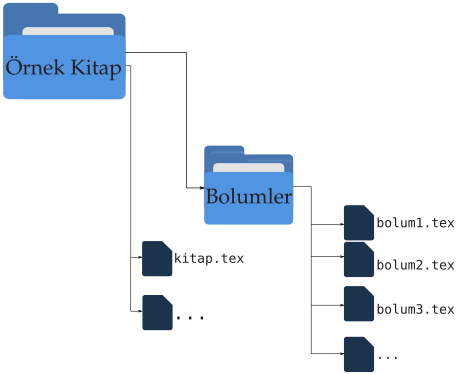
\includegraphics{images/dizin.png}
\caption{Kaynak dosyanın olduğu dizinin
düzenlenmesi}
\end{figure}

Bu şekilde bir düzenleme yaptığınızda \texttt{\textbackslash{}input} ya da \texttt{\textbackslash{}include}
komutlarıyla dosya eklemek istediğinizde dosyanın bulunduğu dizini de
göstermeniz gerekir.

Burada kaynak dosya \texttt{kitap.tex}'dir. Bu kaynak dosyaya \texttt{bolum1.tex}
dosyasını eklemek istediğinizde komutu

\begin{Shaded}
\begin{Highlighting}[]
\NormalTok{\textbackslash{}input\{Bolumler}\SpecialCharTok{/}\NormalTok{bolum1\}}
\end{Highlighting}
\end{Shaded}

şeklinde verirsiniz. Bu sayede kaynak dosyanızın olduğu dizinde (Örnek
Kitap) sadece \texttt{kitap} ile başlayan dosyalar olur. Diğer dosyalar alt
dizinde (Bolumler) yer alır.

Dikkat edilirse ``Örnek Kitap'' dışında, ``Bolumler'' alt dizini ve tüm
dosya adları Türkçe karakter ya da boşluk içermez.

\begin{Shaded}
\begin{Highlighting}[]
\NormalTok{\textbackslash{}documentclass[a4paper,12pt]\{book\}}
\NormalTok{\textbackslash{}usepackage[T1]\{fontenc\}}
\NormalTok{\textbackslash{}usepackage[turkish]\{babel\}}
\NormalTok{\textbackslash{}title\{Örnek Kitap\}}
\NormalTok{\textbackslash{}author\{\textbackslash{}TeX dizgi\}}
\NormalTok{\textbackslash{}begin\{document\}}
\NormalTok{\textbackslash{}frontmatter}
\NormalTok{\textbackslash{}maketitle}
\NormalTok{\textbackslash{}tableofcontents}
\NormalTok{\textbackslash{}input\{Bolumler}\SpecialCharTok{/}\NormalTok{onsoz\}}
\NormalTok{\textbackslash{}mainmatter}
\NormalTok{\textbackslash{}input\{Bolumler}\SpecialCharTok{/}\NormalTok{bolum1\}}
\NormalTok{\textbackslash{}input\{Bolumler}\SpecialCharTok{/}\NormalTok{bolum2\}}
\NormalTok{\textbackslash{}appendix}
\NormalTok{\textbackslash{}input\{Bolumler}\SpecialCharTok{/}\NormalTok{ek1\}}
\NormalTok{\textbackslash{}backmatter}
\NormalTok{\textbackslash{}end\{document\}}
\end{Highlighting}
\end{Shaded}

\hypertarget{varsayux131lan-sayfa-duxfczenini-deux11fiux15ftirme}{%
\section{Varsayılan Sayfa Düzenini Değiştirme}\label{varsayux131lan-sayfa-duxfczenini-deux11fiux15ftirme}}

LaTeX'de varsayılan kağıt boyutunun \texttt{letterpaper} olduğunu Bölün \ref{belgesinifi}'de ifade etmiştik. Ayrıca aynı yazıda başka bir kağıt boyutunun
nasıl seçileceğine de yer vermiştik. Şimdi ise hem sayfamızın kenar
boşluklarının nasıl ayarlanacağından hem de ön tanımlı olmayan, tamamen
keyfi bir sayfa boyutunun nasıl belirleneceğinden bahsedelim.

Bu tür sayfa düzenlemeleri için LaTeX'de
\href{http://ftp.cc.uoc.gr/mirrors/CTAN/macros/latex/contrib/geometry/geometry.pdf}{geometry} paketi kullanılır. Öncelikle paketi

\begin{Shaded}
\begin{Highlighting}[]
\NormalTok{\textbackslash{}usepackage\{geometry\}}
\end{Highlighting}
\end{Shaded}

komutuyla sahanlığa ekleyin. Ardından paket seçeneklerinde aşağıdaki
tanımlamalarla sayfanın düzenini değiştirebilirsiniz:

\begin{longtable}[]{@{}ll@{}}
\toprule
Tanım & Değer \\
\midrule
\endhead
\texttt{top} & üst boșluk \\
\texttt{bottom} & alt boșluk \\
\texttt{left} & sol boșluk \\
\texttt{right} & sağ boșluk \\
\texttt{paperwidht} & sayfa genișliği \\
\texttt{paperheight} & sayfa yüksekliği \\
\bottomrule
\end{longtable}

Örneğin sahanlıkta

\begin{Shaded}
\begin{Highlighting}[]
\NormalTok{\textbackslash{}usepackage[paperwidth}\OtherTok{=}\NormalTok{175mm,paperheight}\OtherTok{=}\NormalTok{255mm,top}\OtherTok{=}\NormalTok{2cm,bottom}\OtherTok{=}\NormalTok{2cm,left}\OtherTok{=}\FloatTok{2.5}\NormalTok{cm,right}\OtherTok{=}\FloatTok{2.5}\NormalTok{cm]\{geometry\}}
\end{Highlighting}
\end{Shaded}

komutunu verdiğinizde boyutu \(175\times 255\) mm, üst ve alt boşluğu
\(2\) cm, sol ve sağ boşluğu \(2.5\) cm olan bir sayfa düzeni
oluşturursunuz. Dilerseniz \texttt{paperwidth} ve\texttt{paperheight} tanımlamalarını
yerine, örneğin \texttt{a4paper} yazarak sadece kenar boşluklarla ilgili
tanımlamaları yapabilirsiniz.

\begin{quote}
LaTeX'de milimetre (mm) ve santimetre (cm) dışında inç (in), punto
(pt), em ve ex gibi ölçü birimleri de vardır. Bunlara ileride
değinilecektir. Ayrıca yine ileride daha ayrıntılı sayfa düzeni
oluşturmaktan da bahsedeceğiz. Bu aşamada bu kadarı yeterli olacaktır.
\end{quote}

\hypertarget{satux131r-ve-sayfa-kesme}{%
\section{Satır ve Sayfa Kesme}\label{satux131r-ve-sayfa-kesme}}

LaTeX, kelimeler arası boşlukları otomatik ayarlayarak satırları iki
yana yaslayarak dizer. Bir satırı kesip yeni bir satıra geçmek için \texttt{\textbackslash{}\textbackslash{}}
veya \texttt{\textbackslash{}newline} komutları kullanılır.

Birinci komut \texttt{\textbackslash{}\textbackslash{}*} şeklinde verildiğinde satırdan sonra sayfa
kesilmesini önler.

Benzer şeyi \texttt{\textbackslash{}linebreak} komutu da yapar. Fakat bu komut ile satır
kesilirse LaTeX kalan yarım satırı iki yana yaslar. \texttt{\textbackslash{}nolinebreak}
komutu ise satırın kesilmesini önler.

Birçok kelimeyi birlikte aynı satırda tutmak gerekirse \texttt{\textbackslash{}mbox} komutu
kullanılır:

\begin{Shaded}
\begin{Highlighting}[]
\NormalTok{\textbackslash{}mbox\{}\SpecialCharTok{\textless{}}\NormalTok{metin}\SpecialCharTok{\textgreater{}}\NormalTok{\}}
\end{Highlighting}
\end{Shaded}

Buradaki \texttt{\textless{}metin\textgreater{}} içindeki kelimeler her durumda birleşik kalırlar.
Benzer şeyi \texttt{\textbackslash{}fbox} komutu da metin etrafına çizgi çizerek yapar.

Sayfayı kesip yeni bir sayfaya geçmek için \texttt{\textbackslash{}newpage} ya da \texttt{\textbackslash{}pagebreak}
komutları kullanılır. \texttt{\textbackslash{}nopagebreak} komutu sayfa kesilmesini önler.
\texttt{\textbackslash{}newpage} ile \texttt{\textbackslash{}pagebreak} komutları arasında da \texttt{\textbackslash{}newline} ile
\texttt{\textbackslash{}linebreak} komutlarındakine benzer bir fark vardır.

\hypertarget{paragraflar-ve-cuxfcmle-sonlarux131}{%
\section{Paragraflar ve Cümle Sonları}\label{paragraflar-ve-cuxfcmle-sonlarux131}}

Boş bir satırın yeni bir paragraf açtığını Bölüm \ref{bosluk}'de belirtmiştik. Aynı şey, \texttt{\textbackslash{}par} komutuyla da yapılabilir.
Ancak bu komut yeni bir paragraf açmaktan ziyade farklı amaçlar için
kullanılır (yeri geldiğinde değinilecektir). Nitekim kaynak dosyanızın
okunabilirliği açısından paragrafları ayırmak için boş bir satır
bırakmak daha kullanışlıdır.

LaTeX'de varsayılan olarak \texttt{\textbackslash{}chapter} ve \texttt{\textbackslash{}section} gibi bölümleme
komutlarından sonra oluşturulan ilk paragraf girintisiz, sonrakiler
girintili olur. Bu, paragraf başlarında \texttt{\textbackslash{}indent} ya da \texttt{\textbackslash{}noindent}
komutlarıyla tek seferliğine değiştirilebilir. Birinci komut girinti
oluşturur, ikincisi ise girintiyi kaldırır.

LaTeX, okumayı kolaylaştırmak için cümle sonlarında fazladan boşluklar
bırakır. Bunu yaparken de her cümlenin nokta, soru işareti veya ünlem
işaretiyle bittiğini varsayar. Kısaltmalarda büyük harflerden sonra
nokta geldiğinden, büyük harften sonra nokta koyulursa LaTeX bunu cümle
sonu saymaz. Eğer bir büyük harften sonra nokta koyuyorsanız ve burası
cümlenin sonuysa LaTeX'in burayı cümle sonu sayması için büyük harften
sonraki noktanın önüne \texttt{\textbackslash{}@} koymanız gerekir.

LaTeX'in noktadan sonra fazladan boşluk \emph{koymamasını} isterseniz
\texttt{\textbackslash{}frenchspacing} komutunu kullanırsınız. Bu komutu kullandıysanız, artık
noktadan önce \texttt{\textbackslash{}@} koymanıza gerek yoktur. Daha sonra tekrar cümle
sonlarında fazladan boşluk kullanmak istenirse de \texttt{\textbackslash{}nonfrenchspacing}
komutu kullanılır.

Unvan kısaltmasından sonra unvanın ait olduğu kelimeyle birlikte kalması
ve fazladan boşluk bırakılmaması için tilda (\texttt{\textasciitilde{}}) işareti
kullanılabilir. Bu işaret hem genişlemeyen bir boşluk bırakır hem de
satırın orada kesilmesini önler.

\hypertarget{aralux131klar}{%
\section{Aralıklar}\label{aralux131klar}}

LaTeX'de hem dikey hem de yatay aralıklar otomatik olarak ayarlanır.
Fazladan aralıklar bırakmak için komutlar kullanılır.

Aralık bırakırken kullanabileceğimiz ölçü birimleri aşağıda
gösterilmiştir.

\begin{longtable}[]{@{}ll@{}}
\toprule
Birim & Değer \\
\midrule
\endhead
mm & milimetre \(\approx 1/25\) inç \\
cm & santimetre = 10 mm \\
in & inç = 25.4 mm \\
pt & punto \(\approx 1/72\) inç \\
em & Kullanılan yazı tipinde `M' harfinin genişliği \\
ex & Kullanılan yazı tipinde `x' harfinin yüksekliği \\
\bottomrule
\end{longtable}

\hypertarget{dikey-aralux131klar}{%
\subsection{Dikey aralıklar}\label{dikey-aralux131klar}}

Dikey aralık birkaç komutla bırakılabilir. Bunlardan biri \texttt{\textbackslash{}vspace}
olup, komut iki boş satır arasında

\begin{Shaded}
\begin{Highlighting}[]
\NormalTok{\textbackslash{}vspace\{}\SpecialCharTok{\textless{}}\NormalTok{uzunluk}\SpecialCharTok{\textgreater{}}\NormalTok{\}}
\end{Highlighting}
\end{Shaded}

şeklinde verilir. Komut bu şekilde verildiğinde komutun zorunlu
değişkeninde birimiyle belirtilen uzunluk kadar dikey aralık bırakılır.
Eğer bir sayfanın başında veya sonunda aralık bırakılmak istenirse,
komut \texttt{\textbackslash{}vspace*} şeklinde yıldızlı vermelidir. Bu komutun aralığa ilave
yapan \texttt{\textbackslash{}addvspace} sürümü de vardır.

Bir paragrafın iki satırı arasında veya bir tablonun satırları arasında
ilave aralık açmak için

\begin{Shaded}
\begin{Highlighting}[]
\NormalTok{\textbackslash{}\textbackslash{}[}\SpecialCharTok{\textless{}}\NormalTok{uzunluk}\SpecialCharTok{\textgreater{}}\NormalTok{]}
\end{Highlighting}
\end{Shaded}

komutu kullanılır.

\begin{Shaded}
\begin{Highlighting}[]
\NormalTok{A\textbackslash{}\textbackslash{}[1ex]}
\NormalTok{B}
\end{Highlighting}
\end{Shaded}

Bu komutlarda belirtilen uzunluklar negatif de olabilir.

\begin{Shaded}
\begin{Highlighting}[]
\NormalTok{A\textbackslash{}\textbackslash{}[}\SpecialCharTok{{-}}\NormalTok{2ex]}
\NormalTok{B}
\end{Highlighting}
\end{Shaded}

Sınırsız bir dikey aralık oluşturmak için \texttt{\textbackslash{}vfill} komutu kullanılır. Bu
komuttan sonra gelen her şey sayfanın altına yaslanır.

Ön tanımlı gelen \texttt{\textbackslash{}smallskip}, \texttt{\textbackslash{}medskip} ve \texttt{\textbackslash{}bigskip} komutları
sırasıyla küçük, orta ve büyük aralıklar bırakır.

\hypertarget{yatay-aralux131klar}{%
\subsection{Yatay aralıklar}\label{yatay-aralux131klar}}

Ön tanımlı yatay aralıklar

\begin{Shaded}
\begin{Highlighting}[]
\NormalTok{\textbackslash{}  \textbackslash{},  \textbackslash{}}\SpecialCharTok{:}\NormalTok{  \textbackslash{};  \textbackslash{}quad  \textbackslash{}qquad  \textbackslash{}}\SpecialCharTok{!}
\end{Highlighting}
\end{Shaded}

komutlarıyla verilir. Bu komutlar sırasıyla bir sözcük arası, \(3/\!18\) em, \(4/\!18\) em, \(5/\!18\) em, \(1\) em, \(2\) em, \(-3/\!18\) em uzunlukta yatay aralık bırakır.

Belli bir uzunlukta yatay aralık bırakmak için \texttt{\textbackslash{}hspace} komutu
kullanılır. Yine dikey aralıkta olduğu gibi yatay aralık negatif de
olabilir. Eğer aralık satır başına veya sonuna rasgelse dahi bu aralığı
korumak istiyorsanız, yıldızlı \texttt{\textbackslash{}hspace*} komutu kullanırsınız.

\begin{Shaded}
\begin{Highlighting}[]
\NormalTok{A\textbackslash{}hspace\{2cm\}B\textbackslash{}\textbackslash{}}
\NormalTok{A \textbackslash{}hspace\{2cm\} B}
\end{Highlighting}
\end{Shaded}

Komutlardan önce veya sonra boşluk bırakmak farklı
sonuçlar üretir.

Sınırsız bir yatay aralık oluşturmak için \texttt{\textbackslash{}hfill} komutu kullanılır. Bu
komuttan sonra gelen her şey satırın sonuna yaslanır. Hem satır sonuna
yaslamak hem de aralığı noktalarla doldurmak isterseniz \texttt{\textbackslash{}dotfill}
komutunu kullanırsınız. Satır sonuna yaslayıp aralığa çizgi çekmek
isterseniz de \texttt{\textbackslash{}hrulefill} komutunu kullanırsınız.

\begin{Shaded}
\begin{Highlighting}[]
\NormalTok{A\textbackslash{}hfill B\textbackslash{}\textbackslash{}}
\NormalTok{A\textbackslash{}dotfill B\textbackslash{}\textbackslash{}}
\NormalTok{A\textbackslash{}hrulefill B}
\end{Highlighting}
\end{Shaded}

\hypertarget{metni-hizalamak-ve-suxfctunlara-buxf6lmek}{%
\section{Metni Hizalamak ve Sütunlara Bölmek}\label{metni-hizalamak-ve-suxfctunlara-buxf6lmek}}

\hypertarget{hizalama}{%
\subsection{Hizalama}\label{hizalama}}

LaTeX'de metni sola hizalamak için \texttt{flushleft}, sağa hizalamak için
\texttt{flushright} ve ortalı hizalamak için \texttt{center} ortamları kullanılır.

\begin{Shaded}
\begin{Highlighting}[]
\NormalTok{\textbackslash{}begin\{flushleft\}}
\NormalTok{ burası sola hizalı}
\NormalTok{\textbackslash{}end\{flushleft\}}
\NormalTok{\textbackslash{}begin\{flushright\}}
\NormalTok{ sağa hizalı}
\NormalTok{\textbackslash{}end\{flushright\}}
\NormalTok{\textbackslash{}begin\{center\}}
\NormalTok{ ve ortalı}
\NormalTok{\textbackslash{}end\{center\}}
\end{Highlighting}
\end{Shaded}

\hypertarget{suxfctunlara-buxf6lmek}{%
\subsection{Sütunlara bölmek}\label{suxfctunlara-buxf6lmek}}

LaTeX'de belgenin tamamının iki sütun dizilmesi için \texttt{\textbackslash{}documentclass}
komutunun seçeneğine \texttt{twocolumn} yazılabileceğinden Bölüm \ref{belgesinifi}'de bahsettik. Bu, tüm belgenin iki sütun dizilmesini sağlar. Bazı
sayfaları iki, bazılarınıysa tek sütun dizmek istiyorsanız \texttt{\textbackslash{}twocolumn}
ve \texttt{\textbackslash{}onecolumn} komutlarını kullanmanız gerekir. \texttt{\textbackslash{}twocolumn} komutunun
verildiği sayfadan sonraki sayfalar iki, \texttt{\textbackslash{}onecolumn} komutunun
verildiği sayfadan sonraki sayfalar tek sütun dizilir.

Eğer metni daha fazla sütuna bölmek ve sütunları istediğiniz yerden
başlatmak gibi daha fazla seçenek istiyorsanız, \texttt{multicols} ortamını
kullanmanız gerekir. Bu ortamı kullanabilmek için

\begin{Shaded}
\begin{Highlighting}[]
\NormalTok{\textbackslash{}usepackage\{multicol\}}
\end{Highlighting}
\end{Shaded}

komutuyla
\href{http://ftp.ntua.gr/mirror/ctan/macros/latex/required/tools/multicol.pdf}{multicol} paketini eklemelisiniz.

\begin{Shaded}
\begin{Highlighting}[]
\NormalTok{\textbackslash{}begin\{multicols\}\{}\SpecialCharTok{\textless{}}\NormalTok{sütun sayısı}\SpecialCharTok{\textgreater{}}\NormalTok{\}}

\NormalTok{\textbackslash{}end\{multicols\}}
\end{Highlighting}
\end{Shaded}

Burada, \texttt{\textless{}sütun\ sayısı\textgreater{}} değişkeninde oluşturulmak istenen sütun adedi
sayıyla belirtilir.

Bu ortamda sütun genişlikleri eşit olup, sütunlar arası boşluk
\texttt{\textbackslash{}columnsep}, sütunlar arasındaki çizginin kalınlığı \texttt{\textbackslash{}columnseprule} ve
sütunlar arasındaki çizginin rengi \texttt{\textbackslash{}columnseprulecolor} komutlarında
saklıdır. Bu değişkenler \texttt{\textbackslash{}setlength} ya da \texttt{\textbackslash{}def} komutları
kullanılarak değiştirilebilir.

\begin{Shaded}
\begin{Highlighting}[numbers=left,,]
\NormalTok{\textbackslash{}setlength\{\textbackslash{}columnsep\}\{1cm\}}
\NormalTok{\textbackslash{}setlength\{\textbackslash{}columnseprule\}\{1pt\}}
\NormalTok{\textbackslash{}def\textbackslash{}columnseprulecolor\{\textbackslash{}color\{blue\}\}}
\end{Highlighting}
\end{Shaded}

Yukarıdaki birinci komutla sütunlar arasındaki boşluk 1 cm, çizgi
kalınlığı 1 pt ve çizgi rengi mavi olarak düzenlenir. Bu komutlar ya
sahanlığa ya da ortamı kullanmadan önce gövdeye yazılmalıdır.

\begin{quote}
Şimdiye kadar renk kullanımından bahsetmedik ancak çizgi rengini
değiştirmek için verilen komutun kullanılabilmesi için sahanlığa
\texttt{\textbackslash{}usepackage\{color\}} komutuyla \texttt{color} paketinin eklenmesi gerekir.
\end{quote}

Ortam isteğe bağlı bir değişken de alabilir. Bu, çengelli parantezlerden
sonra köşeli parantezler içine yazılır. Köşeli parantezler içinde
yazılanlar bölünmeden ve çok sütunlu metnin üstünde dizilir.

\begin{Shaded}
\begin{Highlighting}[]
\NormalTok{\textbackslash{}begin\{multicols\}\{}\DecValTok{2}\NormalTok{\}}
\NormalTok{[\textbackslash{}section\{Başlık\}}
\NormalTok{Burası sütunlara bölünmez.]}
\NormalTok{Burası sütunlara bölünür.}
\NormalTok{\textbackslash{}end\{multicols\}}
\end{Highlighting}
\end{Shaded}

Sütunu kesmek için \texttt{\textbackslash{}columnbreak} komutu kullanılır. Komutun verildiği
yerde sütun kesilir, ardından kesme noktasından önceki paragraflar tüm
kullanılabilir alanı doldurmak için eşit olarak dağıtılır. Dolayısıyla
bazen beklenen sonucu vermeyebilir.

Varsayılan \texttt{multicols} ortamında sütunların her biri aynı miktarda metin
içerecek şekilde dengelenmiştir. Bu, ortamın yıldızlı sürümü
(\texttt{multicols*}) kullanılarak değiştirilebilir.

\hypertarget{listeleme}{%
\section{Listeleme}\label{listeleme}}

\hypertarget{temel-listeler}{%
\subsection{Temel listeler}\label{temel-listeler}}

LaTeX'de listeleme için değişik ortamlar vardır. Bu ortamlar tek başına
kullanılabileceği gibi birlikte de kullanılabilirler. Her ortamda
maddeler \texttt{\textbackslash{}item} komutuyla belirtilir.

Bir listeyi numaralı şekilde dizmek için \texttt{enumerate} ortamı kullanılır.

\begin{Shaded}
\begin{Highlighting}[]
\NormalTok{\textbackslash{}begin\{enumerate\}}
\NormalTok{ \textbackslash{}item madde }\DecValTok{1}
\NormalTok{  \textbackslash{}begin\{enumerate\}}
\NormalTok{    \textbackslash{}item alt madde }\DecValTok{1}
\NormalTok{      \textbackslash{}begin\{enumerate\}}
\NormalTok{        \textbackslash{}item en alt madde }\DecValTok{1}
\NormalTok{      \textbackslash{}end\{enumerate\}}
\NormalTok{    \textbackslash{}item alt madde }\DecValTok{2}
\NormalTok{  \textbackslash{}end\{enumerate\}}
\NormalTok{ \textbackslash{}item madde }\DecValTok{2}
\NormalTok{\textbackslash{}end\{enumerate\}}
\end{Highlighting}
\end{Shaded}

Numarasız, özel işaretli listeler için \texttt{itemize} ortamı kullanılır ve bu
ortamda madde işareti değiştirilebilir.

\begin{Shaded}
\begin{Highlighting}[]
\NormalTok{\textbackslash{}begin\{itemize\}}
\NormalTok{\textbackslash{}item madde }\DecValTok{1}
\NormalTok{\textbackslash{}item madde }\DecValTok{2}
\NormalTok{\textbackslash{}item[}\SpecialCharTok{$}\NormalTok{\textbackslash{}circ}\SpecialCharTok{$}\NormalTok{] madde }\DecValTok{3}
\NormalTok{\textbackslash{}item[}\SpecialCharTok{+}\NormalTok{] madde }\DecValTok{4}
\NormalTok{\textbackslash{}end\{itemize\}}
\end{Highlighting}
\end{Shaded}

Açıklamalı bir liste içinse \texttt{description} ortamı kullanılır. Bu ortamda
köşeli parantez içine alınan anahtar kelimeler kalın dizilir.

\begin{Shaded}
\begin{Highlighting}[]
\NormalTok{\textbackslash{}begin\{description\}}
\NormalTok{\textbackslash{}item[Nokta] Boyutu olmayan}
\NormalTok{\textbackslash{}item[Çember] Bir noktaya eşit}
\NormalTok{uzaklıktaki noktaların geometrik yeri}
\NormalTok{\textbackslash{}end\{description\}}
\end{Highlighting}
\end{Shaded}

\hypertarget{listeleri-uxf6zelleux15ftirmek}{%
\subsection{Listeleri özelleştirmek}\label{listeleri-uxf6zelleux15ftirmek}}

Listelerin özelleştirmek için
\href{http://ftp.ntua.gr/mirror/ctan/macros/latex/required/tools/enumerate.pdf}{enumerate} paketi kullanılabilir. Paketi \texttt{\textbackslash{}usepackage\{enumerate\}}
komutuyla ekledikten sonra \texttt{enumerate} ortamını başlatan komutun peşine
köşeli parantezler içinde madde işaretlerinin tipi belirtilebilir:

\begin{Shaded}
\begin{Highlighting}[]
\NormalTok{\textbackslash{}begin\{enumerate\}[I.]}
\NormalTok{\textbackslash{}item bir}
\NormalTok{\textbackslash{}item iki }
\NormalTok{\textbackslash{}item üç}
\NormalTok{\textbackslash{}end\{enumerate\}}
\end{Highlighting}
\end{Shaded}

Bunun dışında çok daha fazla özelleştirmeye izin veren
\href{http://ftp.cc.uoc.gr/mirrors/CTAN/macros/latex/contrib/enumitem/enumitem.pdf}{enumitem} paketi vardır. Bu paketi kullanarak yapılabilecek
listelere de ilerde değineceğiz. Dileyen okur paket belgesini inceleyip
listelerini özelleştirebilir.

\hypertarget{yazux131tipleri}{%
\section{Yazıtipleri}\label{yazux131tipleri}}

\hypertarget{giriux15f}{%
\subsection{Giriş}\label{giriux15f}}

Yazıtipi konusu \emph{kodlama}, \emph{aile}, \emph{biçem} ve \emph{boyut} olmak üzere dört
alt başlıkta incelenebilir. Kodlama çok teknik bir konu olup amacımız
dışındadır, ancak sadece şunu belirtelim ki kodlama işini LaTeX'de Bölüm \ref{turkce}'de bahsettiğimiz \texttt{fontenc} paketi üstlenir. Bu paketi belgenize eklemiş
olduğunuzu varsayarak devam edeceğiz.

Bu yazıda anlatacağımız şeylerden bazıları bir bakıma LaTeX'in
felsefesine aykırı olacak. Nitekim LaTeX, \texttt{\textbackslash{}documentclass} komutunda
belirtilen ana yazıtipi boyutuna göre, dipnot ya da başlık gibi ana
yazıtipi boyutundan farklı dizilen şeylerin boyutunu olabilecek en güzel
ve doğru şekilde ayarlar. O yüzden bu konudaki klasik uyarıyı biz de
yineleyelim:


\includegraphics{images/uyari.png}

\hypertarget{aile}{%
\subsection{Aile}\label{aile}}

Yazıtipleri Roman ya da Serif, Sans Serif ve Typewriter olmak üzere üç
ailede toplanabilir. Roman ailesi tırnaklı ya da süslü diyebileceğimiz
yazıtiplerini, Sans Serif ailesi tırnaksız ya da süssüz yazıtiplerini ve
Typewriter ailesi de daktilo yazıtiplerini barındırır.

LaTeX'de her belge sınıfı varsayılan yazıtipi ailesiyle gelir. \texttt{beamer}
sınıfının varsayılan ailesi Sans Serif olup, diğer sınıfların varsayılan
ailesi Roman'dır.

Varsayılan aile \texttt{\textbackslash{}familydefault} komutunda saklı olup, \texttt{\textbackslash{}renewcommand}
komutuyla değiştirilebilir.

\begin{Shaded}
\begin{Highlighting}[numbers=left,,]
\NormalTok{\textbackslash{}renewcommand\{\textbackslash{}familydefault\}\{\textbackslash{}rmdefault\}  }
\NormalTok{\textbackslash{}renewcommand\{\textbackslash{}familydefault\}\{\textbackslash{}sfdefault\}  }
\NormalTok{\textbackslash{}renewcommand\{\textbackslash{}familydefault\}\{\textbackslash{}ttdefault\} }
\end{Highlighting}
\end{Shaded}

Birinci komut sahanlığa yazılırsa, belge sınıfından bağımsız olarak
varsayılan aile Roman, ikincisi yazılırsa Sans Serif, üçüncüsü yazılırsa
Typewriter olur.

Eğer belgenin tamamının değilde bazı kelime ya da cümlelerin farklı
aileden yazılması istenirse -- ki genelde böyle kullanılır -- aşağıdaki
komut ya da bildirimler kullanılır.

\begin{figure}
\centering
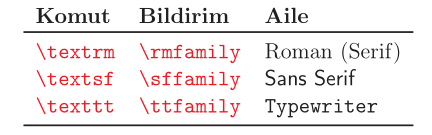
\includegraphics{images/yazitipi.png}
\caption{Yazıtipi
Aileleri}
\end{figure}

LaTeX'de varsayılan yazıtipi Computer Modern olup, ek bir pakete ihtiyaç
duymadan kullanılabilecek yazıtipleri aşağıda gösterilmiştir.

\begin{figure}
\centering
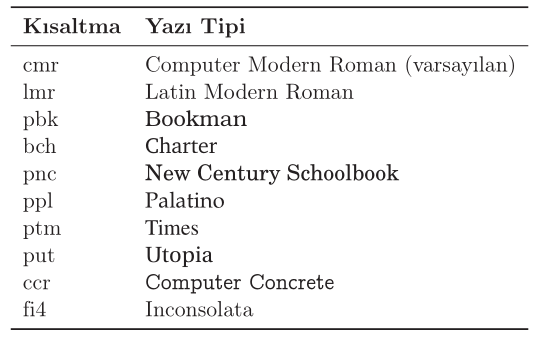
\includegraphics{images/yazitipi2.png}
\caption{Roman
Yazıtipleri}
\end{figure}

\begin{figure}
\centering
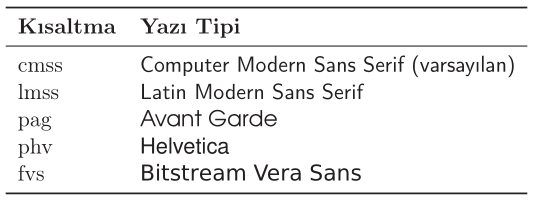
\includegraphics{images/yazitipi3.png}
\caption{Sans Serif
Yazıtipleri}
\end{figure}

\begin{figure}
\centering
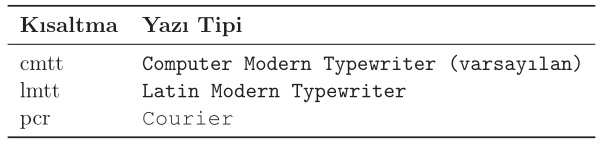
\includegraphics{images/yazitipi4.png}
\caption{Typewriter Yazıtipleri\\
}
\end{figure}

\begin{figure}
\centering
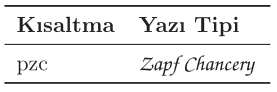
\includegraphics{images/yazitipi5.png}
\caption{Elyazısı}
\end{figure}

Varsayılan yazıtipleri \texttt{\textbackslash{}rmdefault}, \texttt{\textbackslash{}sfdefault} ve \texttt{\textbackslash{}ttdefault}
komutlarında saklı olup, \texttt{\textbackslash{}renewcommand} komutuyla değiştirilebilirler.

\begin{Shaded}
\begin{Highlighting}[]
\NormalTok{\textbackslash{}renewcommand\{\textbackslash{}rmdefault\}\{}\SpecialCharTok{\textless{}}\NormalTok{kısaltma}\SpecialCharTok{\textgreater{}}\NormalTok{\}}
\end{Highlighting}
\end{Shaded}

Burada \texttt{\textless{}kısaltma\textgreater{}}, tablolarda belirtilen kısaltmalardır. Örneğin

\begin{Shaded}
\begin{Highlighting}[]
\NormalTok{\textbackslash{}renewcommand\{\textbackslash{}rmdefault\}\{put\}}
\end{Highlighting}
\end{Shaded}

komutu sahanlığa yazıldığında, eğer varsayılan aile Roman ise belgenizin
ana yazıtipi Utopia olur.

Eğer tüm belgenin değil, bazı kelime ya da cümlelerin farklı yazıtipinde
yazılması istenirse \texttt{\textbackslash{}fontfamily} komutuyla \texttt{\textbackslash{}selectfont} komutu
birlikte aşağıdaki şekilde kullanılır.

\begin{Shaded}
\begin{Highlighting}[]
\NormalTok{\{\textbackslash{}fontfamily\{pbk\}\textbackslash{}selectfont Bookman yazıtipi.\} Ana yazıtipi.}
\end{Highlighting}
\end{Shaded}

Varsayılan yazıtipi paket ekleyerek de değiştirilebilir. Bu hem
pratiktir hem de bazı paketler matematiksel ifadelerin yazıtipine de
etki eder. Bu paketlerin bazıları tabloda gösterilmiştir.

\begin{figure}
\centering
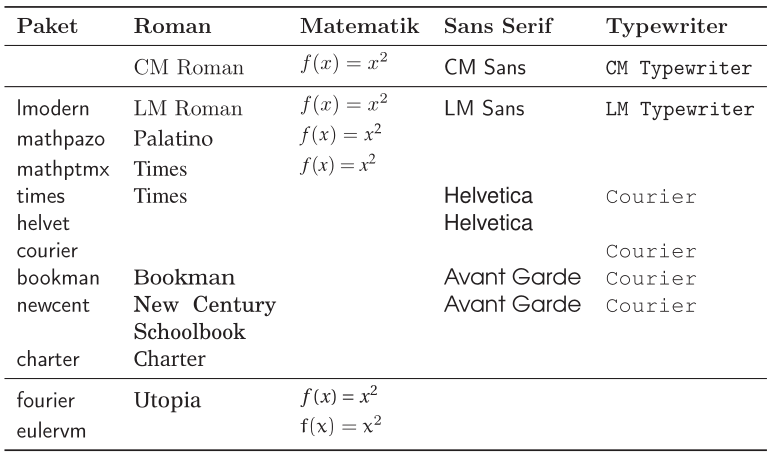
\includegraphics{images/yazitipi6.png}
\caption{Yazıtipi değiştiren
paketler}
\end{figure}

Bunların dışında beğenebileceğiniz birçok yazıtipini \href{https://tug.org/FontCatalogue/}{LaTeX
Yazıtipi
Kataloğu}'nda bulabilirsiniz.

\hypertarget{biuxe7em}{%
\subsection{Biçem}\label{biuxe7em}}

Metin içinde kelimeleri bazen italik bazen de kalın dizmek
isteyebilirsiniz. Bu değişimler aşağıdaki tablodaki komut ya da
bildirimlerle yapılır.

\begin{figure}
\centering
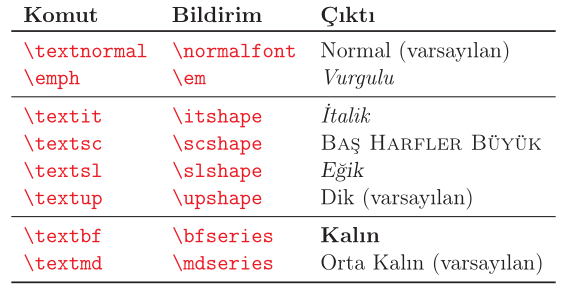
\includegraphics{images/yazitipi7.png}
\caption{Yazıtipi
Biçemleri}
\end{figure}

\begin{Shaded}
\begin{Highlighting}[]
\NormalTok{İzleyen kelime \textbackslash{}textit\{italik\} }
\NormalTok{harflerle yazılmıştır.}
\NormalTok{Metnin geri kalan kısmı}
\NormalTok{normaldir.}
\end{Highlighting}
\end{Shaded}

\href{https://github.com/acarzfr/latex-dersleri/blob/main/examples/ex3.pdf}{Çıktı}

\begin{Shaded}
\begin{Highlighting}[]
\NormalTok{İzleyen ifade \{\textbackslash{}slshape \{\textbackslash{}bfseries eğik kalındır\}\}.}
\end{Highlighting}
\end{Shaded}

\begin{Shaded}
\begin{Highlighting}[]
\NormalTok{İzleyen ifade \textbackslash{}textit\{\textbackslash{}textbf\{italik kalın\}\}, ama bu}
\NormalTok{\textbackslash{}textsc\{\textbackslash{}textit\{büyük küçük harf değil\}\}.}
\end{Highlighting}
\end{Shaded}

Eğer vurgulu metin içinde bazı kelimeler tekrar vurgulanırsa bu
kelimeler normale döner.

\begin{Shaded}
\begin{Highlighting}[]
\NormalTok{\{\textbackslash{}em Vurgulu metinde tekrar}
\NormalTok{vurgu yapılırsa \{\textbackslash{}em normale\}}
\NormalTok{döner.\}}
\end{Highlighting}
\end{Shaded}

LaTeX'de vurgu yukarıdaki gibi yapılsa da altını çizerek vurgu yapmak
isteyen olabilir. Kuyruklu harflerin altı çizildiğinde varsayılan satır
aralığı değiştiğinden vurguyu bu şekilde yapmamanız daha doğrudur. Ancak
illa altını çizmek isterseniz \texttt{\textbackslash{}underline} komutunu kullanabilirsiniz.

\hypertarget{boyut}{%
\subsection{Boyut}\label{boyut}}

Yazıtipi boyutunu değiştirmek için aşağıdaki bildirimler kullanılır.

\begin{figure}
\centering
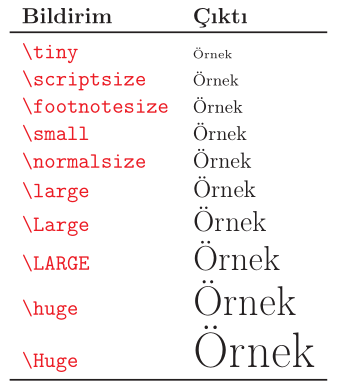
\includegraphics{images/yazitipi8.png}
\caption{Yazıtipi Boyutu Değiştiren
Bildirimler}
\end{figure}

\begin{Shaded}
\begin{Highlighting}[]
\NormalTok{\{\textbackslash{}Large Büyük\} ve}
\NormalTok{\{\textbackslash{}scriptsize küçük\} harfler.}
\end{Highlighting}
\end{Shaded}

Bu bildirimlerin aynı zamanda satır aralığını da değiştirdiğine dikkat
edilmelidir. Aşağıdaki iki örnekte, \texttt{\textbackslash{}par} (paragraf) komutunun
verdiğiniz yere bağlı olarak farklı sonuçlar ürettiği gösterilmiştir.
Doğru kullanım ikincisidir.

\begin{Shaded}
\begin{Highlighting}[]
\NormalTok{\{\textbackslash{}large }
\NormalTok{Sokrates}\SpecialCharTok{:}\NormalTok{ Platon}
\NormalTok{yalan söyleyecek}
\NormalTok{aşağıdaki cümlede.\}\textbackslash{}par}
\end{Highlighting}
\end{Shaded}

\href{https://github.com/acarzfr/latex-dersleri/blob/main/examples/ex4.pdf}{Çıktı}

\begin{Shaded}
\begin{Highlighting}[]
\NormalTok{\{\textbackslash{}large Platon}\SpecialCharTok{:}\NormalTok{ Sokrates}
\NormalTok{doğruyu söyledi}
\NormalTok{önceki cümlede.\textbackslash{}par\}}
\end{Highlighting}
\end{Shaded}

\href{https://github.com/acarzfr/latex-dersleri/blob/main/examples/ex5.pdf}{Çıktı}

Bu bildirimlerin etkisi belge ana yazıtipi boyutuna bağımlıdır. Mutlak
boyutlar aşağıdaki tabloda gösterilmiştir.

\begin{figure}
\centering
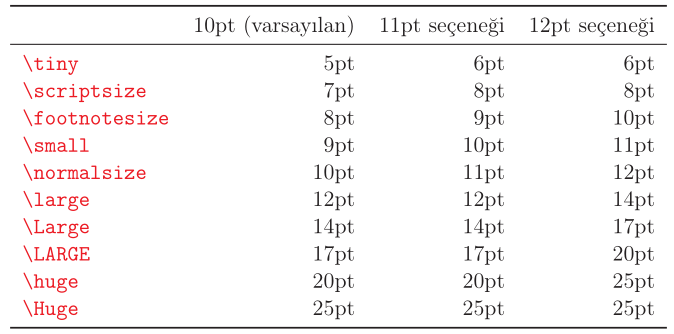
\includegraphics{images/yazitipi9.png}
\caption{Yazıtipleri Mutlak
Boyutları}
\end{figure}

Bağımsız bir yazıtipi boyutu elde etmek için \texttt{\textbackslash{}fontsize} ile
\texttt{\textbackslash{}selectfont} komutları birlikte kullanılır.

\begin{Shaded}
\begin{Highlighting}[]
\NormalTok{\{\textbackslash{}fontsize\{}\SpecialCharTok{\textless{}}\NormalTok{boyut}\SpecialCharTok{\textgreater{}}\NormalTok{\}\{}\SpecialCharTok{\textless{}}\NormalTok{aralık}\SpecialCharTok{\textgreater{}}\NormalTok{\}\textbackslash{}selectfont }\SpecialCharTok{\textless{}}\NormalTok{metin}\SpecialCharTok{\textgreater{}}\NormalTok{\}}
\end{Highlighting}
\end{Shaded}

Buradaki \texttt{\textless{}boyut\textgreater{}} yazıtipi boyutu, \texttt{\textless{}aralık\textgreater{}} ise satır aralığıdır.
İkisinin de ölçü birimi punto (pt) olup, temel kural, aralığın boyutun
\(1.2\) katı olmasıdır.

\begin{Shaded}
\begin{Highlighting}[]
\NormalTok{\{\textbackslash{}fontsize\{}\DecValTok{30}\NormalTok{\}\{}\DecValTok{36}\NormalTok{\}\textbackslash{}selectfont}
\NormalTok{Yazı tipi boyutu }\DecValTok{30}\NormalTok{ punto,}
\NormalTok{satır aralığı }\DecValTok{36}\NormalTok{ punto.\}}
\end{Highlighting}
\end{Shaded}

Ana yazıtipi boyutu \texttt{\textbackslash{}normalsize} komutunda saklı olup, \texttt{\textbackslash{}renewcommand}
komutuyla değiştirilebilir.

\begin{Shaded}
\begin{Highlighting}[]
\NormalTok{\textbackslash{}renewcommand\{\textbackslash{}normalsize\}\{\textbackslash{}fontsize\{}\DecValTok{30}\NormalTok{\}\{}\DecValTok{36}\NormalTok{\}\textbackslash{}selectfont\}}
\end{Highlighting}
\end{Shaded}

Yukarıdaki komutu sahanlığa yazarsanız belgenizin ana yazıtipi boyutu
30 pt, satır aralığı ise 36 pt olur.

\backmatter

  \bibliography{book.bib,packages.bib}

\printindex

\end{document}
